\documentclass[conference]{IEEEtran}

\usepackage{graphicx}
\usepackage{booktabs}
\usepackage{amsmath,amssymb}
\usepackage{array}
\usepackage{multirow}
\usepackage{url}
\usepackage[hidelinks]{hyperref}
\usepackage{xcolor}
\usepackage{enumitem}

\graphicspath{{figures/}}
\setlength{\emergencystretch}{2em}

\title{Robust Sentiment and Emotion Classification on Noisy Urdu Tweets: A Leak-Free Multi-Stage Evaluation on SentiUrdu-1M}

\author{
\IEEEauthorblockN{M. Raqib Hayat and Abu Bakar}
\IEEEauthorblockA{
NUM-BSCS-2022-40 and NUM-BSCS-2022-41\\
Department of Computer Science, Namal University Mianwali\\
CSC-355 Natural Language Processing\\
Instructor: Dr. Muzamil Ahmed\\
Session: 2022--2026 (8th Semester); Submission Date: 20 May 2026}
}

\begin{document}
\maketitle

\begin{abstract}
Urdu sentiment and emotion classification remains difficult because large manually annotated corpora are scarce, social-media writing is noisy and code-mixed, and the largest available datasets rely on weak supervision. This study consolidates a semester-long investigation of SentiUrdu-1M into a leak-aware comparison of classical, neural, and transformer models. The local corpus contains 1,048,000 Urdu tweets, of which 533,429 have usable category labels before cleaning. A deterministic pipeline normalizes Unicode, removes URLs and mentions, retains hashtag text, strips emojis, removes digits and punctuation, and normalizes whitespace. Emoji removal is central: the dataset labels were partly produced from emoticons, so retaining them would allow a classifier to reproduce the labeling heuristic rather than learn Urdu affective language. After empty cleaned texts are removed, 532,661 labeled tweets are divided into a shared stratified 70/15/15 train, validation, and test split. Seven systems are evaluated for three-class sentiment and six-class emotion classification: TF-IDF Logistic Regression and Linear SVM; Text-CNN and BiLSTM with attention using Urdu fastText vectors; and fine-tuned mBERT, XLM-R, and Urdu-RoBERTa. Evaluation uses accuracy, macro precision, macro recall, macro-F1, weighted-F1, and confusion matrices. Linear SVM obtains the highest accuracy on both tasks (approximately 0.878) but has weak macro-F1, revealing majority-class bias. Urdu-RoBERTa achieves the best sentiment macro-F1 (0.4573), while mBERT achieves the best emotion macro-F1 (0.2703). The results show that leakage control and class-sensitive evaluation materially change the interpretation of performance, while weak labels and extreme imbalance remain the main limits to reliable Urdu emotion recognition.
\end{abstract}

\begin{IEEEkeywords}
Urdu NLP, sentiment analysis, emotion classification, weak supervision, label leakage, class imbalance, mBERT, XLM-R, Urdu-RoBERTa
\end{IEEEkeywords}

\section{Introduction}

\subsection{Background and Significance}

Sentiment analysis identifies the polarity expressed in text, whereas emotion classification attempts to distinguish finer affective states such as joy, sadness, anger, fear, disgust, and surprise. These tasks support public-opinion monitoring, customer feedback analysis, policy assessment, crisis communication, and social-science research. For Urdu-speaking communities, however, many practical systems either ignore Urdu content or apply models developed for English. Such transfer is unreliable because Urdu differs in script, morphology, available lexical resources, and social-media conventions.

Urdu is written in a right-to-left Arabic-derived script and is frequently mixed with English or Roman Urdu online. Tweets also contain inconsistent spellings, decorative symbols, URLs, mentions, hashtags, emojis, and compressed or poetic language. Negation scope and sarcasm can invert literal polarity, while a single sentence may contain multiple emotional cues. These properties make the task a language-understanding problem rather than a direct keyword lookup.

The data problem is equally important. Small manually annotated Urdu corpora provide cleaner labels but limited coverage. SentiUrdu-1M was introduced to address scale through weak supervision, using emoticons and lexical signals to automatically label more than one million tweets \cite{ghafoor2023sentiurdu}. Weak supervision reduces annotation cost, yet it creates systematic noise: labels may disagree with the linguistic content, rare classes receive few examples, and the labeling cues themselves can remain inside the model input. A model that reads the same emoji used to create a label can report impressive accuracy without understanding the Urdu text. This is a form of target leakage and is the central methodological risk addressed in this work.

\subsection{Research Problem and Motivation}

The research problem is to determine how classical machine learning, deep neural networks, and pretrained multilingual or Urdu-specific transformers compare on the same large, noisy Urdu tweet corpus when preprocessing, splits, weighting, and evaluation are held constant and emoji-derived label leakage is explicitly blocked. The problem includes two related tasks:

\begin{enumerate}[leftmargin=*,nosep]
    \item three-class sentiment classification into Negative, Neutral, and Positive; and
    \item six-class emotion classification into Joy, Sad, Angry, Fear, Disgust, and Surprise.
\end{enumerate}

The motivation is both practical and scientific. A robust Urdu classifier could improve local-language monitoring for institutions and researchers. Scientifically, the project tests whether sophisticated contextual encoders provide meaningful gains once a shortcut feature is removed and once extreme imbalance is evaluated with macro-F1 rather than accuracy alone.

\subsection{Objectives, Scope, and Contributions}

The study has four objectives: (1) characterize the local SentiUrdu-1M files and label quality; (2) construct a deterministic leak-free preprocessing and label-canonicalization pipeline; (3) compare seven models from three families under an identical experimental protocol; and (4) analyze not only aggregate scores but also minority-class behavior and common linguistic errors.

The realized contributions are:

\begin{itemize}[leftmargin=*,nosep]
    \item a reproducible eight-stage Urdu tweet cleaning pipeline that removes emojis before feature extraction;
    \item canonicalization of 298 non-null raw category surface forms into six emotion labels and a documented mapping to three sentiment labels;
    \item a controlled comparison of TF-IDF, fastText-based neural networks, and three transformer encoders on the same split;
    \item an analysis showing why high accuracy can coexist with poor class-balanced performance; and
    \item saved predictions, leaderboards, confusion matrices, and visual diagnostics supporting the reported findings.
\end{itemize}

The scope is limited to the local SentiUrdu-1M files and the two classification tasks. The manually verified gold test set proposed at the beginning of the semester was not completed and is therefore treated as future work. The final submission includes a lightweight Streamlit interface for leakage-aware preprocessing and local inference with the packaged Linear SVM model; saved outputs support inspection of the more expensive model families. The remainder of the paper reviews related research, presents the methodology, describes the dataset and experiment, discusses results, and concludes with limitations and future directions.

\section{Related Work}

\subsection{Classical and Lexicon-Based Approaches}

Early Urdu and Roman-Urdu sentiment work was shaped by small datasets and limited pretrained resources. Bilal \emph{et al.} compared Naive Bayes, decision trees, and k-nearest neighbors on 300 Roman-Urdu and English blog opinions, establishing a simple bag-of-words baseline but offering little evidence of generalization \cite{bilal2016roman}. Nasim and Ghani modeled Urdu tweet polarity through Markov chains, adding local sequence information beyond bag-of-words features \cite{nasim2020markov}. Mukhtar and Khan combined an Urdu sentiment lexicon with rules for negation, intensification, and conjunction, demonstrating the value of linguistic structure but remaining bounded by lexicon coverage and out-of-vocabulary text \cite{mukhtar2020lexicon}.

The broader survey by Khattak \emph{et al.} found recurring weaknesses across Urdu sentiment research: inconsistent preprocessing, nonstandard datasets, binary labels, and limited reproducibility \cite{khattak2021survey}. Muhammad and Burney later compared machine and deep-learning techniques on symmetric two-class social-media datasets, but the balanced binary design does not reflect the rare neutral and emotion classes encountered in naturally collected tweets \cite{muhammad2023innovations}. Work on the related Arabic ASTD corpus showed how an approximately 10,000-tweet benchmark could support four-way subjectivity and sentiment evaluation, while also exposing imbalance as a central issue in right-to-left social-media NLP \cite{nabil2015astd}.

These studies support the inclusion of transparent TF-IDF baselines in the present work. They also demonstrate why classical accuracy is not sufficient: sparse lexical models can be competitive on a dominant class while missing the context, morphology, and minority labels that define the harder problem.

\subsection{Deep Neural Approaches}

Dense embeddings and sequence models expanded Urdu sentiment analysis beyond feature engineering. Ashraf \emph{et al.} introduced a six-emotion, multi-label Urdu tweet dataset and evaluated classical models, CNNs, LSTMs, hybrid CNN-LSTM systems, and BERT, using multi-label measures such as macro-F1 and Hamming loss \cite{ashraf2022multilabel}. Their work is especially relevant because it emphasizes emotion classification and class-sensitive metrics, although its 6,043 manually labeled tweets are much smaller than SentiUrdu-1M.

For Roman Urdu, a faster recurrent convolutional architecture improved sentiment classification over rule-based and conventional recurrent baselines on RUSA-19 \cite{nagra2022faster}. Khan \emph{et al.} evaluated traditional, recurrent, convolutional, and multilingual BERT models on 9,312 manually annotated Urdu reviews; mBERT reached an F1 score of 81.49\%, but the curated review domain is cleaner than Twitter \cite{khan2022multiclass}. Sehar \emph{et al.} combined dependency rules with a neural classifier for concept-level Urdu sentiment, illustrating that explicit syntax can help when domain-specific rules are available \cite{sehar2023hybrid}. A stacked CNN-BiLSTM architecture with attention and multilingual BERT embeddings later achieved strong results on UCSA datasets \cite{khan2025empowering}.

Resource construction also remained important. Samreen and Ali built Roman-Urdu emotion and mood resources through lexicon transliteration and automatic annotation, but their labels inherit lexicon and matching errors \cite{samreen2024dataset}. Across 22 multilingual tweet datasets, Barreto \emph{et al.} found that contextual representations often outperform static or count-based features, while the size of the gain depends on dataset and domain match \cite{barreto2023assessment}. These findings motivate the Text-CNN and BiLSTM branches in the current comparison and caution against assuming that a model ranking from clean reviews will transfer to weakly labeled tweets.

\subsection{Transformer, Weakly Supervised, and Multimodal Work}

SentiUrdu-1M is the central large-scale resource for this project. Ghafoor \emph{et al.} collected 1,140,821 tweets and proposed weak labels derived from emoticons and SentiWordNet, comparing the scheme with VADER and TextBlob \cite{ghafoor2023sentiurdu}. The public local file used here contains 1,048,000 rows, a difference discussed in Section IV. The source work solves the scale problem but leaves label quality and leakage as open concerns.

Narejo \emph{et al.} explicitly fused emoji embeddings with mBERT and XLM-R representations on SentiUrdu-1M, reporting text-only accuracy near 64--65\% and much higher values for some emoji-fusion settings \cite{narejo2024emoji}. Those results show that emojis are predictive, but because emoticons participated in label creation, they also sharpen the leakage concern. For this reason, the present system removes emojis rather than using them as features.

Transformer hybrids have also been used for Urdu sarcasm detection, where mBERT, BiLSTM, and multi-head attention outperformed non-transformer baselines on a manually re-annotated tweet corpus \cite{hassan2024sarcasm}. On cleaner Urdu blog data, fine-tuned mBERT achieved 96.5\% accuracy \cite{saeed2024indepth}; this is not directly comparable to weakly labeled Twitter data but illustrates the influence of label and domain quality. Weakly supervised aspect-based sentiment methods use seed words and self-training to exploit unlabeled Urdu tweets, though they risk propagating early errors \cite{zoya2023weakly}.

Domain-adapted pretraining is another promising direction. XLM-T continues XLM-R pretraining on multilingual Twitter and generally improves over generic XLM-R on tweet tasks, although Urdu was not included in its main eight-language sentiment benchmark \cite{barbieri2022xlmt}. Multimodal multilingual research such as M2SA combines text and images and finds that sentiment-specialized text encoders remain strong, with image features helping selected ambiguous cases \cite{thakkar2024m2sa}.

\subsection{Research Gap}

The reviewed literature leaves three connected gaps. First, many Urdu studies use clean but small corpora, while large weakly labeled corpora are less often evaluated with strict leakage controls. Second, cross-paper comparisons mix datasets, preprocessing rules, splits, and metrics. Third, high accuracy is frequently reported without sufficient emphasis on class-balanced performance. This project addresses these gaps by removing emoji cues, using one shared split, comparing three model families, and treating macro-F1 and confusion matrices as primary evidence. It does not fully solve label quality because no independent gold test set is available; instead, that limitation is made explicit.

\section{Proposed Methodology}

\subsection{End-to-End Workflow}

Figure~\ref{fig:architecture} shows the implemented system. Raw tweets are cleaned deterministically, labels are canonicalized, and the labeled data is split once. Each example then follows one of three representation/model branches. All branches produce a sentiment or emotion prediction and are evaluated on the same test rows.

\begin{figure*}[t]
    \centering
    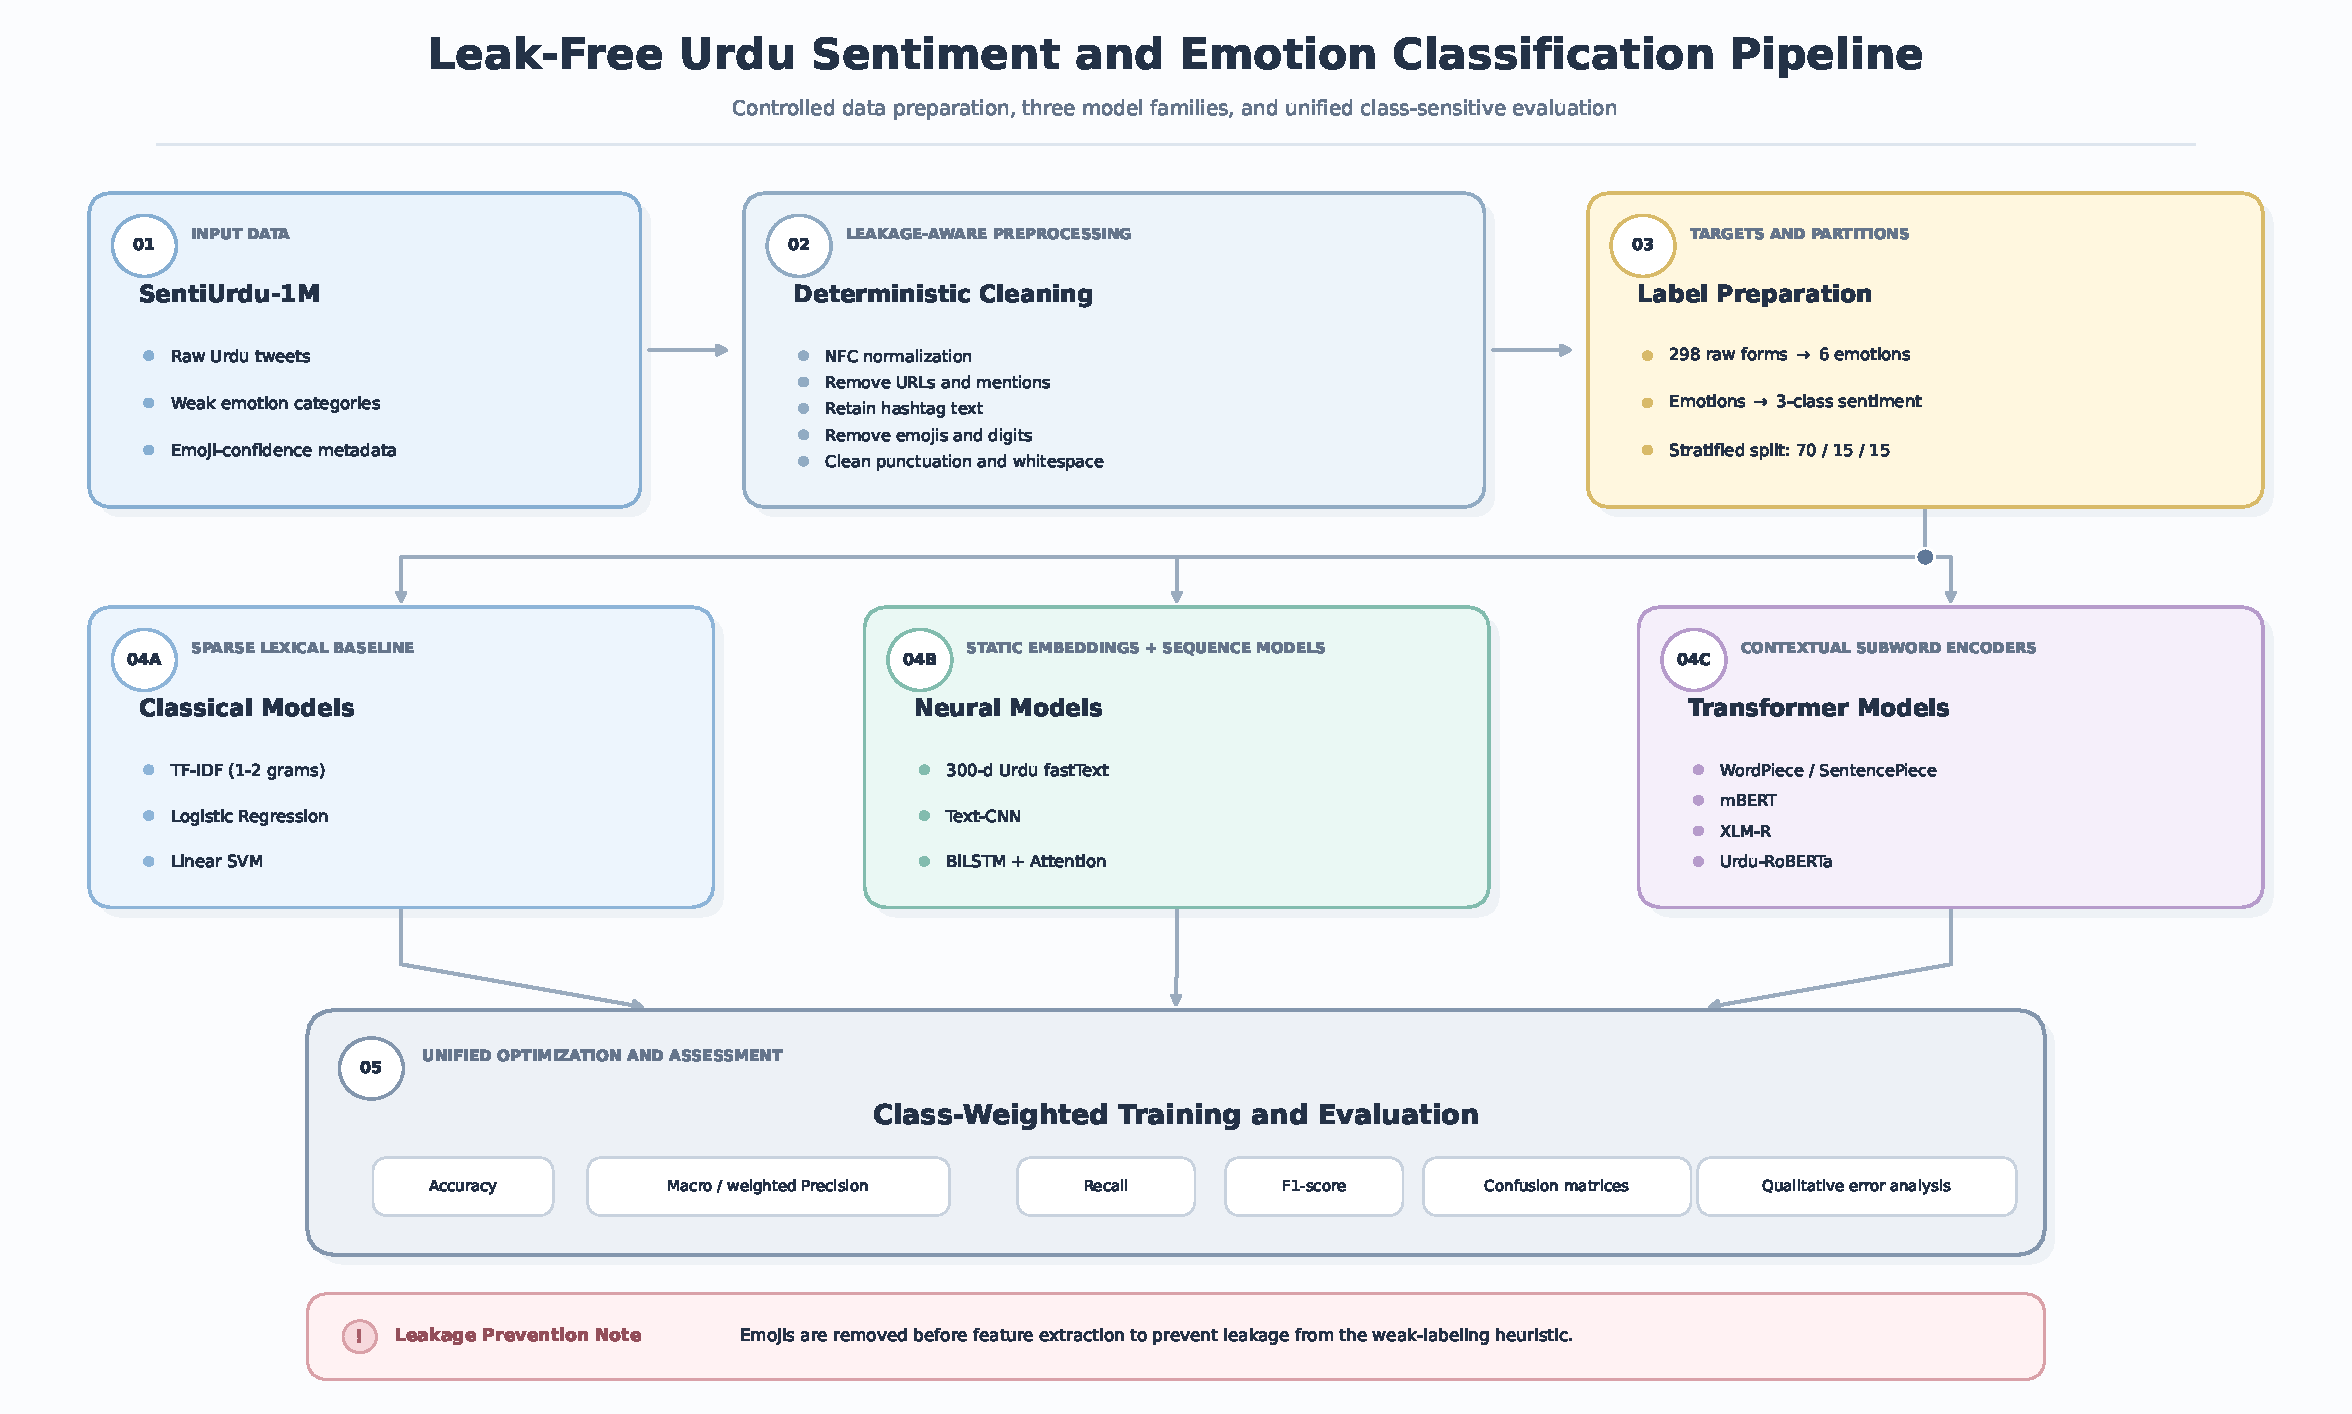
\includegraphics[width=0.98\textwidth]{system_architecture.pdf}
    \caption{Overview of the proposed leak-free Urdu sentiment and emotion classification pipeline.}
    \label{fig:architecture}
\end{figure*}

\subsection{Preprocessing and Leakage Control}

For a raw tweet $x$, preprocessing applies the composition
\begin{equation}
T(x)=t_8(t_7(\cdots t_2(t_1(x))\cdots)),
\end{equation}
where the eight transformations are NFC normalization, URL removal, mention removal, hashtag-symbol removal, emoji removal, digit removal, punctuation removal, and whitespace normalization. Hashtag words are preserved because they may carry topic or sentiment information. Lowercasing is not applicable to Urdu script. Stemming, lemmatization, and universal stop-word deletion are avoided because reliable Urdu tools were not established in the project and transformers require contextual function words.

Emoji removal is the defining control. Let $E(x)$ be the emoji set in $x$ and let $y$ be a label partially produced by a function of those emojis. Training on $E(x)$ risks learning $\hat{y}\approx f(E(x))$ instead of linguistic evidence in $T(x)$. The pipeline enforces $E(T(x))=\emptyset$. Figure~\ref{fig:leakage} shows the strong conditional association observed between raw emoji-derived sentiment and category labels, which justifies removal.

\begin{figure}[t]
    \centering
    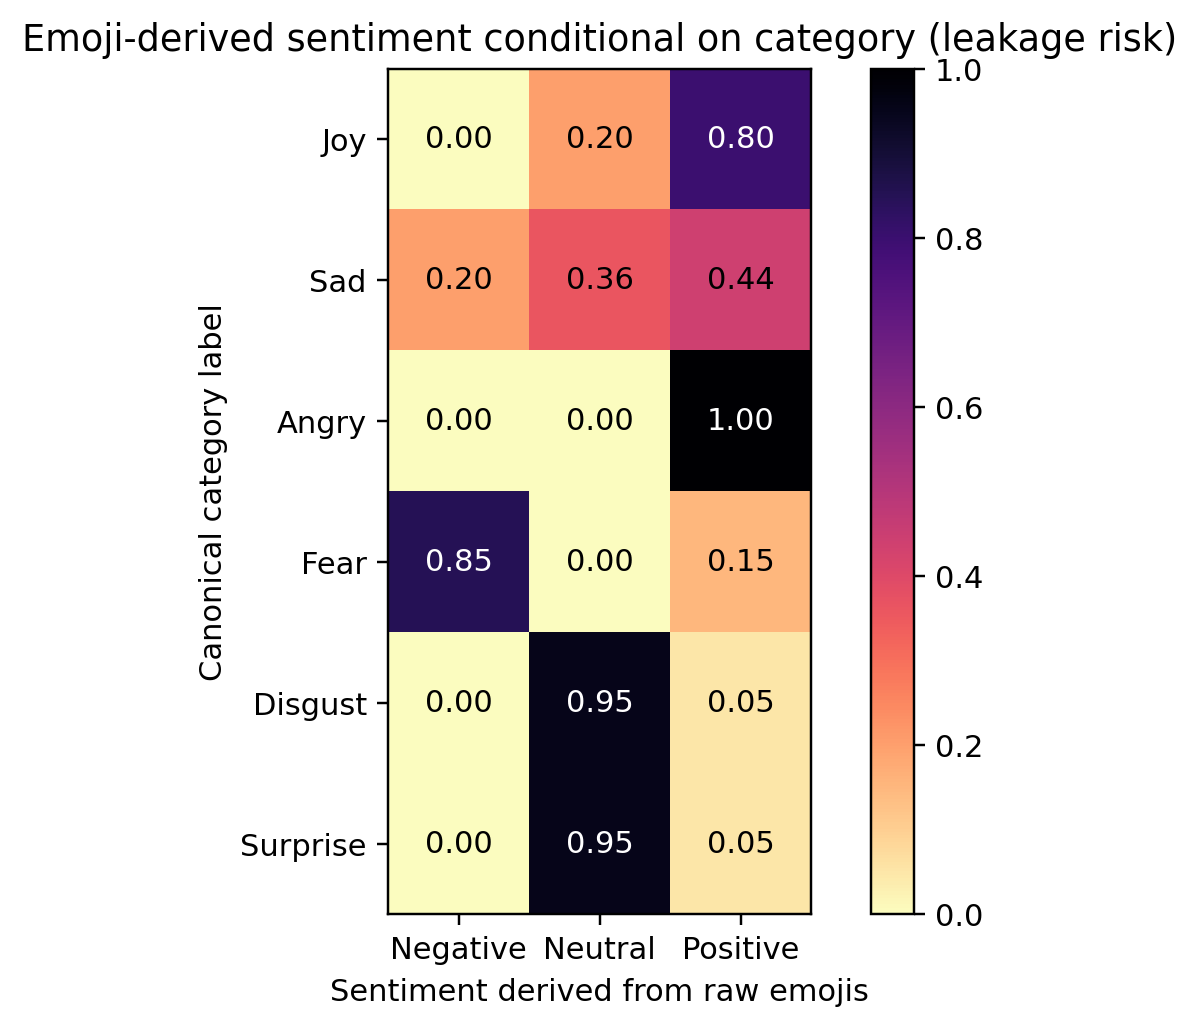
\includegraphics[width=\columnwidth]{label_leakage_heatmap.png}
    \caption{Conditional association between sentiment derived from raw emojis and canonical categories in the Assignment 3 diagnostic. Strong cells indicate a shortcut risk if emojis remain in the input.}
    \label{fig:leakage}
\end{figure}

\subsection{Label Canonicalization and Tasks}

The raw `Category' column contains leading spaces, list-like strings, repeated labels, multi-label cells, and the misspelling `Surprice.' Parsing extracts recognized labels and maps them to Joy, Sad, Angry, Fear, Disgust, or Surprise. Multi-label cells are reduced by majority vote, with corpus-frequency tie breaking. This produces the six-class emotion target.

The three-class sentiment target is derived deterministically: Joy maps to Positive; Sad, Angry, Fear, and Disgust map to Negative; and Surprise maps to Neutral. This mapping is a project design decision grounded in the available labels. It also creates a very small neutral class, so the sentiment task remains highly imbalanced.

\subsection{Classical Models}

The classical branch converts cleaned tweets into TF-IDF vectors with unigram and bigram features. For term $w$ in document $d$,
\begin{equation}
\mathrm{tfidf}(w,d)=\left(1+\log c_{w,d}\right)
\log\left(\frac{1+N}{1+\mathrm{df}(w)}\right),
\end{equation}
followed by vector normalization. The vocabulary is capped at 50,000 features with minimum document frequency 3. Logistic Regression uses the `saga' solver, $C=1$, balanced class weights, and at most 1,000 iterations. Linear SVM uses $C=1$, balanced class weights, and a 2,000-iteration limit. These models provide efficient and interpretable lexical baselines using scikit-learn \cite{pedregosa2011sklearn}.

\subsection{Deep Neural Models}

The neural branch tokenizes cleaned text by whitespace, retains up to 80,000 vocabulary items, truncates sequences to 64 tokens, and initializes 300-dimensional embeddings from Urdu fastText vectors \cite{mikolov2018fasttext}. Unknown vectors are randomly initialized and embeddings remain trainable.

The Text-CNN follows the sentence-classification design of Kim \cite{kim2014cnn}. Parallel one-dimensional convolutions with widths 3, 4, and 5 use 128 filters each. Max-over-time pooling yields fixed-size features, followed by dropout 0.5 and a linear output layer.

The second model is a two-layer bidirectional LSTM \cite{hochreiter1997lstm} with hidden size 256 per direction and dropout 0.4. Additive attention \cite{bahdanau2015attention} assigns a learned weight $\alpha_t$ to each hidden state $h_t$:
\begin{align}
e_t&=v^\top\tanh(Wh_t+b),\\
\alpha_t&=\frac{\exp(e_t)}{\sum_j\exp(e_j)},\qquad
s=\sum_t\alpha_t h_t.
\end{align}
The sentence vector $s$ is passed to the classification layer. Both neural models use Adam with learning rate $10^{-3}$, batch size 256, up to eight epochs, gradient clipping, and early stopping with patience 2.

\subsection{Transformer Models}

The transformer branch fine-tunes mBERT (`bert-base-multilingual-cased'), XLM-R (`xlm-roberta-base'), and Urdu-RoBERTa (`urduhack/roberta-urdu-small'). BERT learns bidirectional contextual representations through masked-language-model pretraining \cite{devlin2019bert}; XLM-R scales cross-lingual representation learning \cite{conneau2020xlmr}; and RoBERTa modifies the BERT training recipe for stronger pretraining \cite{liu2019roberta}. All rely on multi-head self-attention introduced by Vaswani \emph{et al.} \cite{vaswani2017attention}.

Tweets are subword-tokenized and truncated to 96 tokens. A new linear classification head is trained with the encoder. mBERT and XLM-R use learning rate $2\times10^{-5}$ and batch size 32; Urdu-RoBERTa uses $3\times10^{-5}$ and batch size 64. Each is trained for three epochs with AdamW, weight decay 0.01, warmup ratio 0.06, dynamic padding, and mixed precision when CUDA is available.

\subsection{Class-Weighted Objective and High-Level Algorithm}

All model families use inverse-frequency class weighting. For class $k$ with $n_k$ samples among $N$ examples and $K$ classes, the weight is
\begin{equation}
w_k=\frac{N}{K n_k}.
\end{equation}
The weighted cross-entropy loss is
\begin{equation}
\mathcal{L}=-\frac{1}{B}\sum_{i=1}^{B}w_{y_i}\log p(y_i\mid x_i).
\end{equation}

\begin{figure}[t]
\centering
\fbox{\parbox{0.93\columnwidth}{
\textbf{Algorithm 1: Shared training and evaluation procedure}
\begin{enumerate}[leftmargin=*,nosep]
\item Load the local CSV and inspect schema and missing labels.
\item Apply the eight deterministic cleaning operations.
\item Discard empty cleaned tweets; canonicalize emotion and derive sentiment.
\item Build a stratified 70/15/15 split with seed 42 for each task.
\item Compute class weights from the training labels.
\item For each representation/model branch, fit on training data and select using validation macro-F1.
\item Predict the untouched shared test split.
\item Save predictions and compute accuracy, macro precision/recall/F1, weighted-F1, and confusion matrices.
\item Compare model families and inspect representative errors.
\end{enumerate}}}
\caption{High-level pseudocode of the experimental workflow.}
\label{alg:workflow}
\end{figure}

\section{Dataset and Experimental Setup}

\subsection{Source, Local Files, and Data Characteristics}

SentiUrdu-1M is a public Urdu Twitter resource created through weak supervision \cite{ghafoor2023sentiurdu}. The paper reports 1,140,821 collected tweets. The local project CSV used for all experiments contains 1,048,000 rows and four columns: tweet ID, text, an emoji-confidence list, and category. The accompanying workbook has a 1,048,000-row first sheet plus a second sheet, but the implementation consistently reads the CSV and does not merge the sheets.

Of the 1,048,000 CSV rows, 514,571 have a missing category and 533,429 have a non-null category before text cleaning. The cleaning process removes 1,172 rows whose content becomes empty, leaving 532,661 examples for both tasks. The final split is 372,862 training, 79,899 validation, and 79,900 test examples.

Figure~\ref{fig:distribution} and Table~\ref{tab:distribution} show the canonical emotion distribution before empty-text removal. Joy accounts for 86.2\% of labeled rows; Surprise and Fear each contribute less than 0.4\%. The imbalance ratio between Joy and Surprise is approximately 296:1. The derived sentiment distribution is similarly skewed: Positive 459,728, Negative 72,149, and Neutral 1,552 before empty-text removal.

\begin{figure}[t]
    \centering
    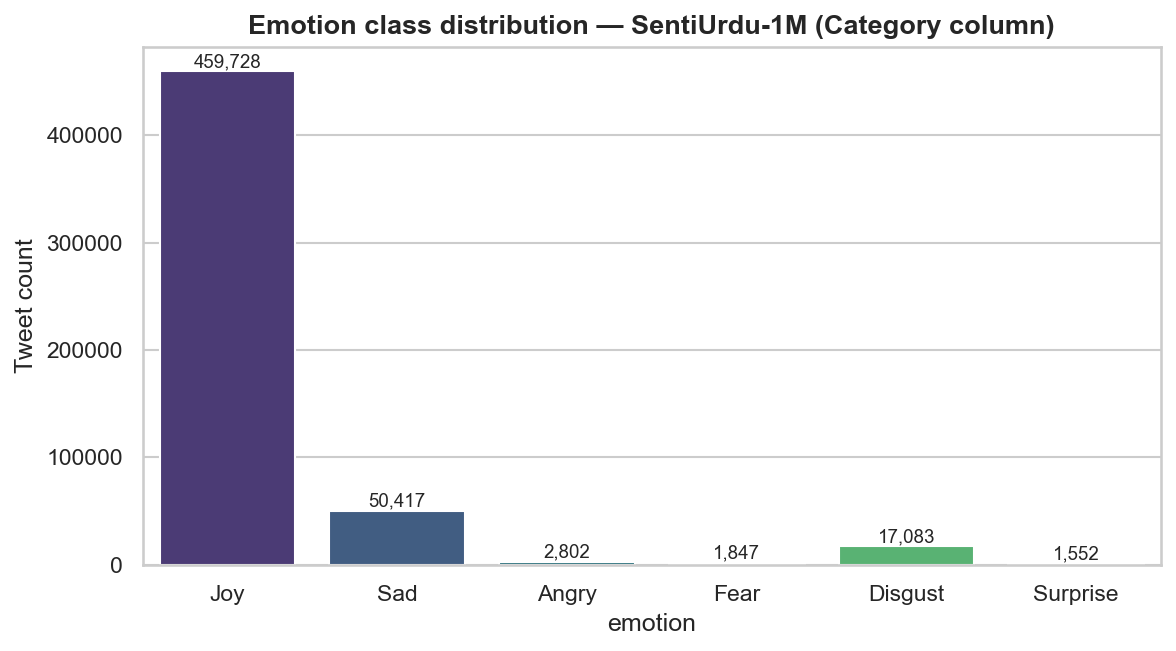
\includegraphics[width=\columnwidth]{emotion_distribution.png}
    \caption{Canonical emotion distribution in the labeled local corpus before empty-cleaned-text removal.}
    \label{fig:distribution}
\end{figure}

\begin{table}[t]
\caption{Canonical Emotion Distribution}
\label{tab:distribution}
\centering
\footnotesize
\begin{tabular}{lrr}
\toprule
Class & Count & Share (\%) \\
\midrule
Joy & 459,728 & 86.2 \\
Sad & 50,417 & 9.5 \\
Disgust & 17,083 & 3.2 \\
Angry & 2,802 & 0.5 \\
Fear & 1,847 & 0.3 \\
Surprise & 1,552 & 0.3 \\
\bottomrule
\end{tabular}
\end{table}

Tweets have a cleaned median length of approximately 11 tokens and a reported 95th percentile near 36 tokens. The project therefore uses length 64 for word-level neural models and 96 subwords for transformers. An audit reported substantial emoji, URL, mention, hashtag, and Latin-script content, supporting task-specific cleaning rather than generic English preprocessing.

\subsection{Software, Hardware, and Reproducibility}

The implementation uses Python, pandas, NumPy, scikit-learn, PyTorch, Hugging Face Transformers/Datasets, emoji, regex, matplotlib, seaborn, and Jupyter. The project metadata targets Python 3.10--3.12. Assignment 3 records an NVIDIA RTX 5070 Ti with 16 GB VRAM, CUDA 12.8, driver 581.57, PyTorch 2.12 development build with CUDA 12.8, and Transformers 4.57.x. CPU and RAM specifications were not recorded. Reported runtimes were approximately 1--2 minutes for classical fitting, 5--10 minutes per CNN/BiLSTM model, and 60--90 minutes per transformer for three epochs.

Random seed 42 is set for Python, NumPy, PyTorch, scikit-learn splits, and Hugging Face training. Every saved prediction file contains the same 79,900 test examples for a task. The experiment does not include repeated seeds, confidence intervals, or statistical significance tests, so small differences should not be overinterpreted.

\subsection{Evaluation Metrics}

For class $k$, precision and recall are
\begin{equation}
P_k=\frac{TP_k}{TP_k+FP_k},\qquad
R_k=\frac{TP_k}{TP_k+FN_k},
\end{equation}
and $F1_k=2P_kR_k/(P_k+R_k)$. Macro-F1 averages $F1_k$ equally across classes, whereas weighted-F1 weights each class by support. Accuracy measures the overall correct fraction. Because Joy/Positive dominates the corpus, macro-F1 is the principal comparative measure; accuracy and weighted-F1 are reported to expose the effect of class prevalence. Row-normalized confusion matrices show recall patterns for every true class.

\section{Results and Discussion}

\begin{table*}[t]
\caption{Three-Class Sentiment Classification Results on the Shared Test Split}
\label{tab:sentiment-results}
\centering
\footnotesize
\setlength{\tabcolsep}{7pt}
\begin{tabular}{lccccc}
\toprule
Model & Accuracy & Macro Precision & Macro Recall & Macro F1 & Weighted F1 \\
\midrule
Logistic Regression & 0.6598 & 0.4046 & 0.4372 & 0.3852 & 0.7107 \\
Linear SVM          & \textbf{0.8783} & \textbf{0.5620} & 0.3848 & 0.4004 & \textbf{0.8409} \\
Text-CNN            & 0.7848 & 0.4407 & 0.5413 & 0.4533 & 0.8117 \\
BiLSTM-Attention    & 0.7762 & 0.4350 & \textbf{0.5424} & 0.4500 & 0.8040 \\
mBERT               & 0.8054 & 0.4748 & 0.4807 & 0.4526 & 0.8217 \\
XLM-R               & 0.7897 & 0.5120 & 0.4894 & 0.4475 & 0.8118 \\
Urdu-RoBERTa        & 0.7750 & 0.4492 & 0.5019 & \textbf{0.4573} & 0.8011 \\
\bottomrule
\end{tabular}
\end{table*}

\begin{table*}[t]
\caption{Six-Class Emotion Classification Results on the Shared Test Split}
\label{tab:emotion-results}
\centering
\footnotesize
\setlength{\tabcolsep}{7pt}
\begin{tabular}{lccccc}
\toprule
Model & Accuracy & Macro Precision & Macro Recall & Macro F1 & Weighted F1 \\
\midrule
Logistic Regression & 0.3601 & 0.2530 & 0.2994 & 0.1632 & 0.4959 \\
Linear SVM          & \textbf{0.8773} & \textbf{0.4517} & 0.1989 & 0.2087 & \textbf{0.8347} \\
Text-CNN            & 0.6476 & 0.2435 & 0.3700 & 0.2499 & 0.7215 \\
BiLSTM-Attention    & 0.6064 & 0.2420 & \textbf{0.3721} & 0.2428 & 0.6910 \\
mBERT               & 0.6922 & 0.2635 & 0.3219 & \textbf{0.2703} & 0.7467 \\
XLM-R               & 0.6907 & 0.2545 & 0.3043 & 0.2535 & 0.7462 \\
Urdu-RoBERTa        & 0.6153 & 0.2503 & 0.3500 & 0.2539 & 0.6971 \\
\bottomrule
\end{tabular}
\end{table*}


\subsection{Sentiment Classification}

Table~\ref{tab:sentiment-results} reports the three-class results. Linear SVM obtains the highest accuracy (0.8783) and weighted-F1 (0.8409), but its macro-F1 is only 0.4004. Urdu-RoBERTa obtains the best macro-F1, 0.4573, followed closely by Text-CNN (0.4533), mBERT (0.4526), and BiLSTM-Attention (0.4500). The absolute difference between Urdu-RoBERTa and Text-CNN is 0.0040, which is too small to claim a robust superiority without repeated runs.

The result changes depending on the metric. Accuracy favors the model that best captures the Positive majority. Macro-F1 favors models that trade some majority accuracy for Negative and Neutral coverage. Even the best sentiment system has weak Neutral recall. In the best Urdu-RoBERTa confusion matrix, only 6\% of true Neutral examples are predicted Neutral; 42\% are predicted Negative and 52\% Positive. This is unsurprising because the test split contains only 232 Neutral examples compared with 68,856 Positive examples.

\subsection{Emotion Classification}

Table~\ref{tab:emotion-results} shows a more difficult six-class problem. Linear SVM again reaches the highest accuracy (0.8773), yet its macro-F1 falls to 0.2087 because it predicts Joy for nearly all minority examples. mBERT achieves the strongest macro-F1 at 0.2703, ahead of Urdu-RoBERTa (0.2539), XLM-R (0.2535), and Text-CNN (0.2499). The best transformer advantage over Text-CNN is approximately 0.0204 macro-F1: meaningful in the observed leaderboard, but still modest relative to the remaining error.

The mBERT confusion matrix in Fig.~\ref{fig:confusions} reveals the minority-class bottleneck. Joy recall is 0.73 and Sad recall is 0.58, but Angry recall is 0.17, Fear 0.10, Disgust 0.31, and Surprise 0.05. Half or more of Angry, Fear, and Surprise examples are predicted Joy. Class weighting encourages minority predictions, but it cannot create reliable linguistic evidence when labels are scarce and noisy.

\begin{figure*}[t]
    \centering
    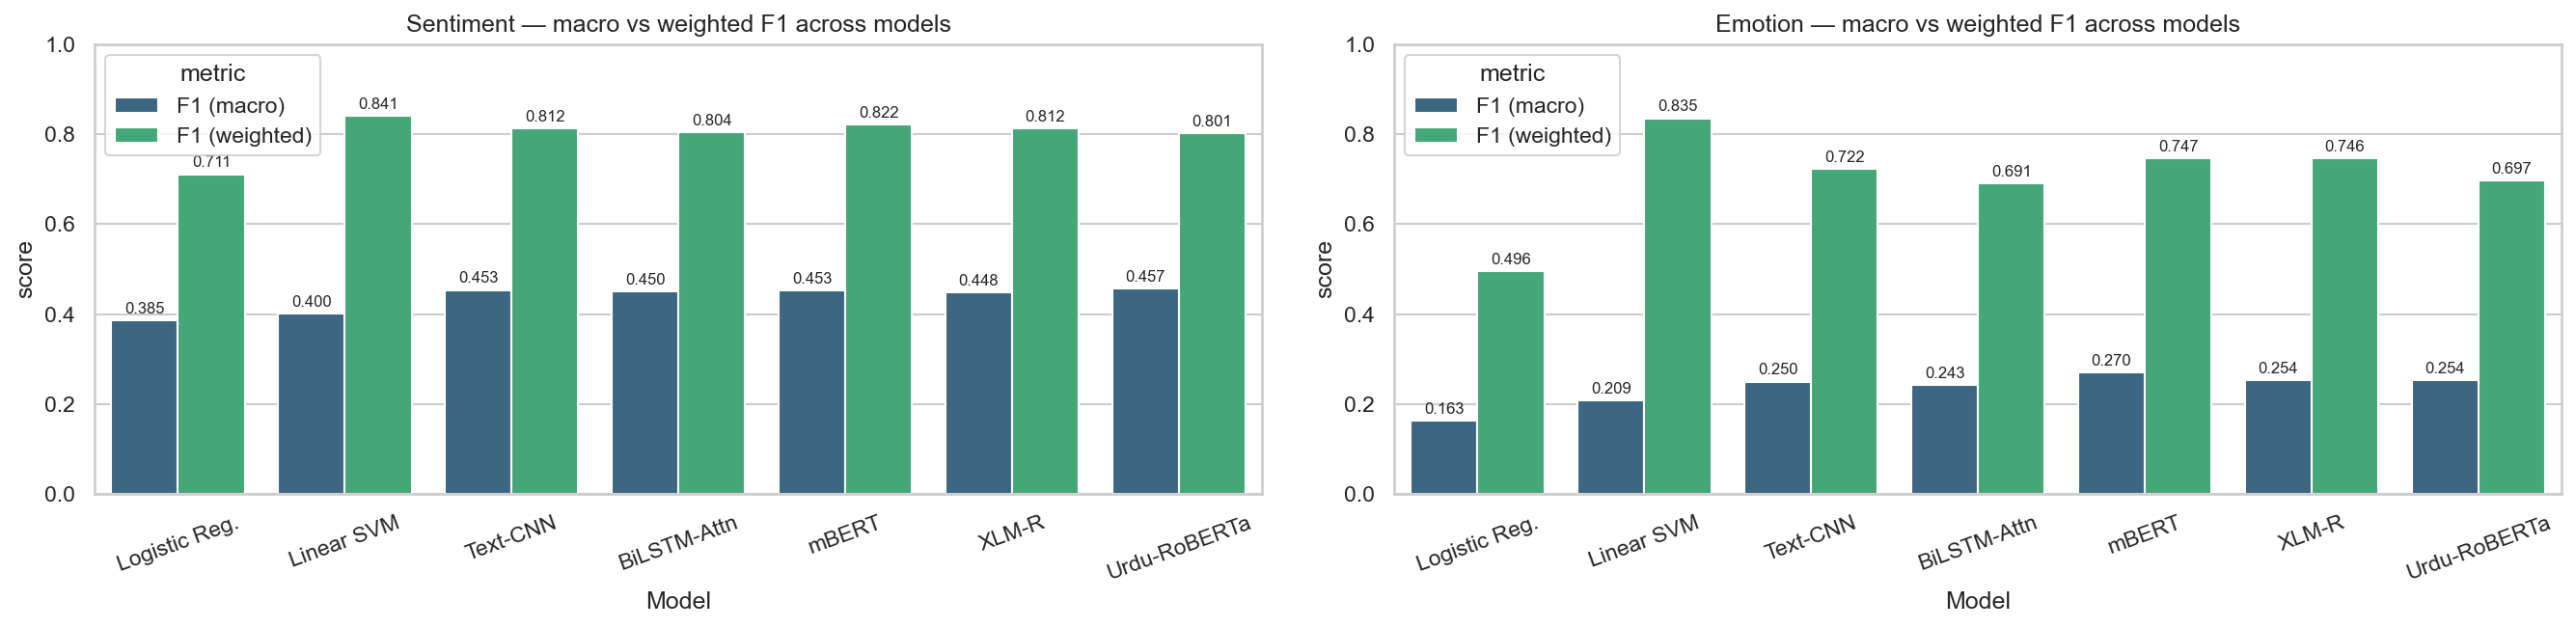
\includegraphics[width=0.92\textwidth]{f1_comparison.png}
    \caption{Macro-F1 versus weighted-F1. The large gaps, especially for Linear SVM, show that strong majority-class performance does not imply balanced classification.}
    \label{fig:f1comparison}
\end{figure*}

\begin{figure*}[t]
    \centering
    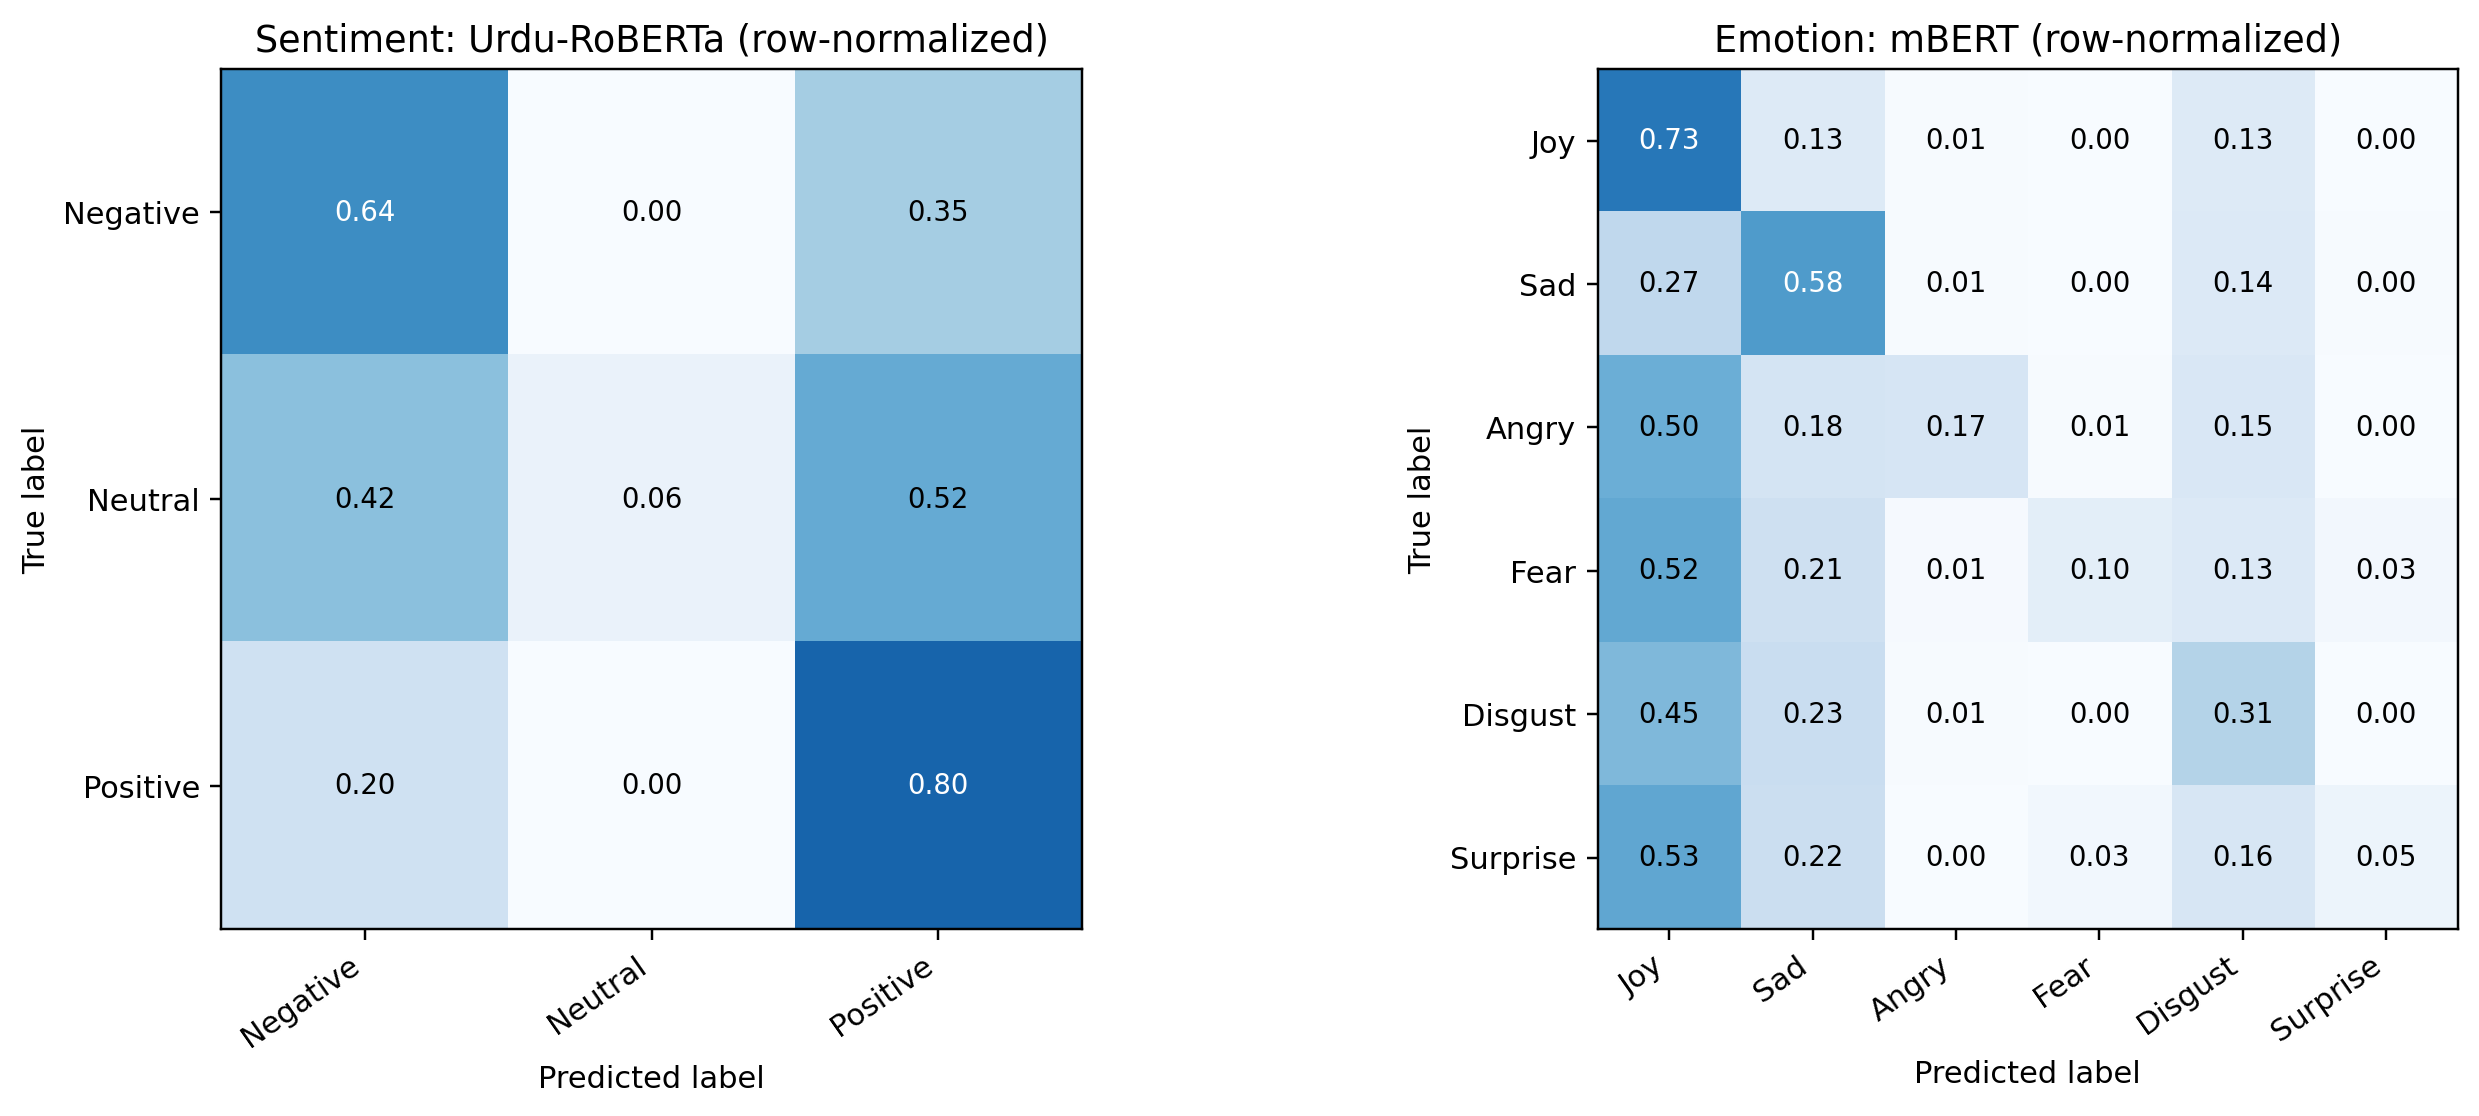
\includegraphics[width=0.88\textwidth]{best_model_confusions.png}
    \caption{Row-normalized confusion matrices for the best macro-F1 system on each task: Urdu-RoBERTa for sentiment and mBERT for emotion.}
    \label{fig:confusions}
\end{figure*}

\subsection{Macro Versus Weighted Performance}

Figure~\ref{fig:f1comparison} makes the imbalance effect explicit. Linear SVM has a sentiment weighted-F1 of 0.8409 but macro-F1 of 0.4004; on emotion the gap expands from 0.8347 weighted-F1 to 0.2087 macro-F1. A deployment judged only by accuracy or weighted-F1 could therefore appear strong while failing most rare emotional states.

Logistic Regression makes the opposite trade-off. Balanced weights and the softer decision boundary encourage minority predictions, increasing recall for some classes but generating many false positives. Its emotion accuracy falls to 0.3601 and macro-F1 to 0.1632. The neural and transformer models occupy a more useful middle ground: lower headline accuracy than SVM, but higher and more stable macro-F1.

\subsection{Comparison of Model Families}

The observed ordering does not support a simple claim that transformers dominate. On sentiment, Text-CNN and BiLSTM are essentially tied with the transformer group. Urdu fastText embeddings provide strong language-specific lexical information, while short tweet length makes local convolutional features competitive. On emotion, mBERT provides the best macro-F1, suggesting that contextual subwords help separate some ambiguous classes, but the gain is limited by labels rather than architecture alone.

Urdu-specific pretraining is also not uniformly decisive. Urdu-RoBERTa leads sentiment but trails mBERT on emotion. XLM-R is close to both. Model capacity, pretraining corpus size, tokenizer coverage, optimization, and the interaction between class weighting and noisy labels may matter as much as the nominal language specialization.

Comparison with literature must remain cautious. mBERT results above 80\% F1 on curated Urdu reviews \cite{khan2022multiclass} and 96.5\% accuracy on clean blog data \cite{saeed2024indepth} do not contradict the lower scores here; they reflect cleaner labels and different domains. Similarly, emoji-fusion accuracy on SentiUrdu-1M \cite{narejo2024emoji} answers a different question because emoji features overlap with the weak-label process. The present experiment deliberately accepts lower apparent scores in exchange for a stricter text-only evaluation.

\subsection{Error Analysis and Influencing Factors}

The Assignment 3 qualitative analysis identifies several recurrent errors. First, negation terms can reverse otherwise positive phrases, but TF-IDF does not reliably model their scope. Second, sarcasm often expresses negative intent through superficially positive words, a known challenge even for transformer hybrids \cite{hassan2024sarcasm}. Third, Latin-script code-mixing fragments the vocabulary and can cause sparse models to fall back to common classes. Fourth, religious and poetic Urdu may contain intense emotional language while receiving a Joy label from the weak heuristic. Finally, very short or context-dependent tweets lack enough lexical evidence after emojis are removed.

Three dataset factors dominate the results. (1) Weak labels impose an unknown noise ceiling and can encode cultural or topical biases. (2) The extreme class distribution makes rare-class learning statistically difficult. (3) the label mapping from emotion to sentiment creates a Neutral class from Surprise alone, producing only 232 Neutral test examples after cleaning and splitting. The confusion matrices and macro/weighted gaps are therefore not incidental artifacts; they are direct consequences of the task construction.

\subsection{Validity and Limitations of the Results}

The experiment has several threats to validity. The test set is stratified but not manually re-annotated, so it measures agreement with weak labels rather than verified human affect. All results use one fixed seed, and small model differences may change under retraining. The local CSV contains fewer rows than the source paper reports, and the second workbook sheet is not integrated. The domain is Pakistani Twitter and may not transfer to reviews, news, or formal Urdu. The original Assignment 3 artifact tree did not include cached splits or model checkpoints; the final submission now packages processed splits, classical checkpoints, saved predictions, metrics, and figures, while large neural and transformer weight files remain excluded. These limitations constrain the strength of causal claims but do not invalidate the central comparison among the saved outputs.

\section{Conclusion and Future Work}

This project investigated sentiment and emotion classification for noisy Urdu tweets under weak supervision. It consolidated an eight-stage preprocessing pipeline, canonicalized noisy labels, and compared seven classical, neural, and transformer systems on a shared stratified split. The key design choice was to remove emojis before feature extraction, preventing models from exploiting a cue used by the labeling heuristic.

The results demonstrate why metric selection matters. Linear SVM achieved approximately 0.878 accuracy on both tasks but weak macro-F1, indicating majority-class collapse. Urdu-RoBERTa achieved the best three-class sentiment macro-F1 of 0.4573, while mBERT achieved the best six-class emotion macro-F1 of 0.2703. Neural fastText models remained close to transformers, showing that architecture alone cannot overcome label noise and 296:1 imbalance. The main contribution is therefore not a single high score, but a controlled, leak-aware evaluation that makes model limitations visible.

Future work should first construct a native-speaker gold test set and report inter-annotator agreement. Repeated-seed experiments and bootstrap confidence intervals are needed before interpreting small leaderboard gaps. Noise-robust losses, active learning, self-training on the 514,571 unlabeled-category rows, focal loss, balanced sampling, and calibrated thresholding may improve minority recall. Domain-adapted models such as XLM-T \cite{barbieri2022xlmt}, parameter-efficient fine-tuning, cross-corpus evaluation, and explicit code-mixing or sarcasm modules are also promising. The included Streamlit interface can be extended with calibrated uncertainty, token-level explanations, and restored deep-model checkpoints for a more complete responsible deployment.

\bibliographystyle{IEEEtran}
\bibliography{references}

\end{document}
